\chapter{Exploratory data analysis of phase diagrams}\label{chapter4}
Organic thin films made of conjugated polymers and/or small molecules have captured the interest of the organic electronics industry due to their wide range of alterable properties (e.g., the color of light emission and solubility in organic solvents). 
High-performing devices have recently been designed with a multi-component material system (as opposed to initial studies that focused on binary blends). 
This reaffirmed the need for a holistic approach to materials design beyond binary blends used to understand the mixing behavior and morphology formation during the fabrication of multi-component organic thin films.

In this chapter, we present a thermodynamics based framework to identify the suitable solvents for a solvent-based manufacturing of organic blends. We present high throughput exploration and construction of a composition-phase diagram map that captures thermodynamics characteristics and facilitates understanding of the multi-component solution's mixing behavior. Our analysis pipeline consists of (i)~a thermodynamics based model to determine phase diagrams of multi-component mixtures using the convex hull method; and (ii)~high throughput analysis of a large set of phase diagrams using dimensionality reduction coupled with the clustering. To illustrate our pipeline, we derive the design rules for material systems typically
used in organic thin films.
\section{Introduction}
Organic thin films made of conjugated polymers and/or small molecules have captured the interest of the organic electronics industry due to their wide range of alterable properties (e.g., color of light emission and solubility in organic solvents). 
Of those properties, solubility crucially facilitates solution-based polymer processing from the liquid phase, making the materials ideal for rapid, inexpensive, large-scale, low-temperature roll-to-roll fabrication. 
Other important properties are flexibility, stretchability, softness, and compatibility with biological systems, all of which are typically absent in conventional silicon-based solutions. 
For these reasons, organic thin films have the potential to revolutionize the next generation of electronic devices within a wide array of technologies, including organic transistors, organic solar cells (OSC), and implantable medical devices and sensors.
At the current state-of-the-art, multiple processing variants exist (e.g., spin coating, doctor blading, casting, roll-to-roll manufacturing), as well as multiple variants tailored for specific materials systems (e.g., blend of polymers and small molecules).  
This proliferation of processing variants is driven by the realization that small changes in the processing can significantly improve a device's performance. 
Classic examples include changing solvents~\cite{Shaheen2001} and adding thermal annealing as a post-processing step, which have together generated organic solar cells with efficiency increased by two orders of magnitude. 
However, processing variants have been all chosen as a result of trial-and-error approaches. 
Consequently, it has remained challenging to establish reliable generalizations of material-process-morphology relationships that can be used to invert those relationships and inform new solvent-based manufacturing variant design.
In this chapter, we use the phase diagram as a representation of the thermodynamics characteristics with the goal of deriving the design rules for solvent selection in organic solar cells. 

Organic Solar Cells~(OSC), the direct application for this work, typically consists of a donor and acceptor materials sandwiched between two electrodes.
Conjugated polymer is typically selected as an electron donor, fullerene (or another polymer) is typically selected as an acceptor. 
OSC are manufactured using various methods of which we are interested in solvent based techniques where donor and acceptor polymers are mixed in a volatile solvent(s)~\cite{krebs2009fabrication}. 
During the manufacturing process, the solvent evaporates to form the morphology. 
Solvent evaporation directs the morphology evolution, and the choice of the solvent is of high importance for the final efficiency of the devices~\cite{Shaheen2001}. 
The first step towards understanding the formation of various phases in the presence of evaporating solvent (of mixture of solvents) is to study the thermodynamics of polymer mixtures. 
In this area, only recently figures of merit have been introduced to capture some characteristics of mixing behavior~\cite{ye2018miscibility}, and to establish a relationship with device properties, followed by derivation of the initial design rules~\cite{ye2018}. Also, features of phase diagrams been included in the reasoning about fabrication of OSC performance~\cite{tashvigh2015novel,li2011determination}, resulting in some initial success. 

In this chapter, we focus on the phase diagram of multi-component material system.
CALPHAD software~\cite{sundman2015opencalphad} is the most widely used tool to study phase diagrams in multi-component systems, but it focuses mostly on alloys. 
Similarly, in the area of fluid multi-component systems, similar approaches have emerged only recently~\cite{SoftMatterCEM,voskov2015ternapi}. 
In the area of organic blends, the phase diagrams of polymeric, or small molecule, multi-component material systems have been analyzed only up to ternaries~\cite{NBB07,li2011determination}. 
This is because the phase diagram construction for multi-component systems has high computational complexity. 
For example, the computational complexity of the equilibrium determination based on convex envelope method (CEM) is
\(\mathcal{O}(N_{\phi}^{(N-1)N/2})\), where \(N\) is the number of components and \(N_{\phi}\) is the number of grid points per each component~\cite{SoftMatterCEM,voskov2015ternapi}.

In this chapter, the CEM method introduced in~\cite{OryllCEM,SoftMatterCEM} is used due to its reasonable computational cost up to
quaternary systems.
We focus on material systems under fixed pressure and temperature, and aim to determine the number of phases for a given a given multi-nary composition.
CEM involves finding the equilibrium compositions of a multi-component system that can be understood by studying the Gibbs free energy landscape~\cite{GibbsCriteria1}. 
A global minimum of the Gibbs free energy landscape determines a true equilibrium state of the system while a meta-stable region is determined by local minima~\cite{OryllCEM,TangentPlaneCriteria,GibbsCriteria1}. 
CEM computes a map of composition space to its corresponding stable phases, given a free energy landscape~(comprising of composition as coordinates and energy as the height value).
The resulting map from CEM when visualized in the composition coordinates-- referred to as the \textit{phase diagram}--reveals the coexisting phases as a function of composition~\cite{SoftMatterCEM}.

We are interested in a high-throughput generation and analysis of material phase diagrams.
In particular, for solvent based OSC manufacturing, a series of experiments needs to be performed in order to select a good solvent for a given set of molecules.
This greatly limits the ability to search and evaluate large amount of solvents in a high-throughput manner.
Alternatively, one can use a phase diagram as a signature of a thermodynamic compatibility of a solvent when mixed with the set of conjugated polymers.
Techniques borrowed from machine learning allows us to study phase diagrams as points in a high-dimensional data space and analyze multiple phase diagrams together using multi-variate approaches.   
In this chapter, multi-variate approaches are used to identify subgroups in phase diagrams, obtain lower dimensional representations of the data space, that are useful in understanding statistical design rules for solvent selection. 

The rest of the chapter is arranged as follows: in \Cref{sec:cem} the convex envelope method~(CEM) to obtain a phase diagram is explained; then the CEM is applied in a high-throughput manner to generate large data sets described in \Cref{sec:htedata}; The data analysis framework is presented in \Cref{sec:pipeline} for the phase diagrams data sets and derivation of data-driven design rules for solvent selection in organic blend manufacturing are demonstrated in \Cref{sec:results}.    

\section{Methods}
\subsection{Phase diagram generation}\label{sec:cem}
Gibbs phase stability states that a globally stable equilibrium state can be obtained by constructing (lower) convex hull of energy over composition~\cite{OryllCEM,SoftMatterCEM}. 
A phase diagram can be determined by applying Gibbs stability criteria of energy landscape~\cite{GibbsCriteria1} using the convex envelope method~(CEM) introduced in~\cite{OryllCEM,SoftMatterCEM}.
According to Gibbs rules, stable compositions lie on the convex hull of energy landscape while unstable compositions lie above.
The CEM is generic and can be applied to any given energy function form. 
Two forms of energy functions are evaluated: polynomial and Flory-Huggins.
The later is used to study the multi-component organic blend system and is defined using the generalized form for an \(N\) component system given by~\Cref{eq:FH}. 
\begin{equation}\label{eq:FH}
    f_{\text{FH}} = \sum_{i=1}^{N}  \frac{1}{M_i} \phi_{i}\lnn{\phi_i} + \sum_{i=1}^{N}\sum_{j(\neq i)=1}^{N}\phi_i \phi_j \chi_{ij}
\end{equation}
where \(\phi\) is composition defined in terms of volume fraction , \(N\) is total number of components in the mixture, \(\chi_{ij}\) are Flory-Huggins interaction parameters between components \(i,j\) and \(M_i\) is degree of polymerization of \(i^{th}\) compound. 

A step-by-step procedure of CEM is described below and an example is shown in~\Cref{fig:workflow} for a three component system (i.e. \(N=3\)).
\begin{enumerate}\label{algo:cem}
    \item[Input:] Free energy function, desired mesh size
    \item[1.] \textbf{Grid generation:} Create a grid \(G\) using an user-defined mesh size $N_{\phi}$ (in terms of number of points per component/dimension) as an n-dimensional hyperplane of compositions (volume fractions \(\{\phi_i\}_{i=1}^{n}\)).
    \item[2.] \textbf{Compute free energy landscape:} Evaluate free energy at each point in \(G\). This results in a (discrete) energy landscape. 
    \item[3.] \textbf{Compute convex envelope:} Compute the convex hull of energy landscape. 
    \item[4.] \textbf{Lower convex hull}: Obtain a lower convex hull~\footnote{Given a energy landscape as a set of points and a height function (energy) , one can obtain the lower convex hull by first adding a point at infinity height to the set and then excluding the simplices that connect to it.} and project it to \(G\) by simply looking up the vertex indices resulting in a mesh of \(G\). 
    The outcome from this step is the projected lower hull, \(G_l\), where vertices corresponds to the points in \(G\).
    \item[5.] \textbf{Compute phase labels:} For each simplex in the mesh $G_l$, assign a phase label based on the number of connected components (as described in~\cite{SoftMatterCEM}). 
    An user defined threshold \(\Delta\) is used to compute adjacency matrix which in turn is used to compute number of connected components.
    \item[Output:] Phase diagram represented as $G_l$ with the phase label assigned to each simplex. 
\end{enumerate}

\begin{figure}[h]
    \centering
    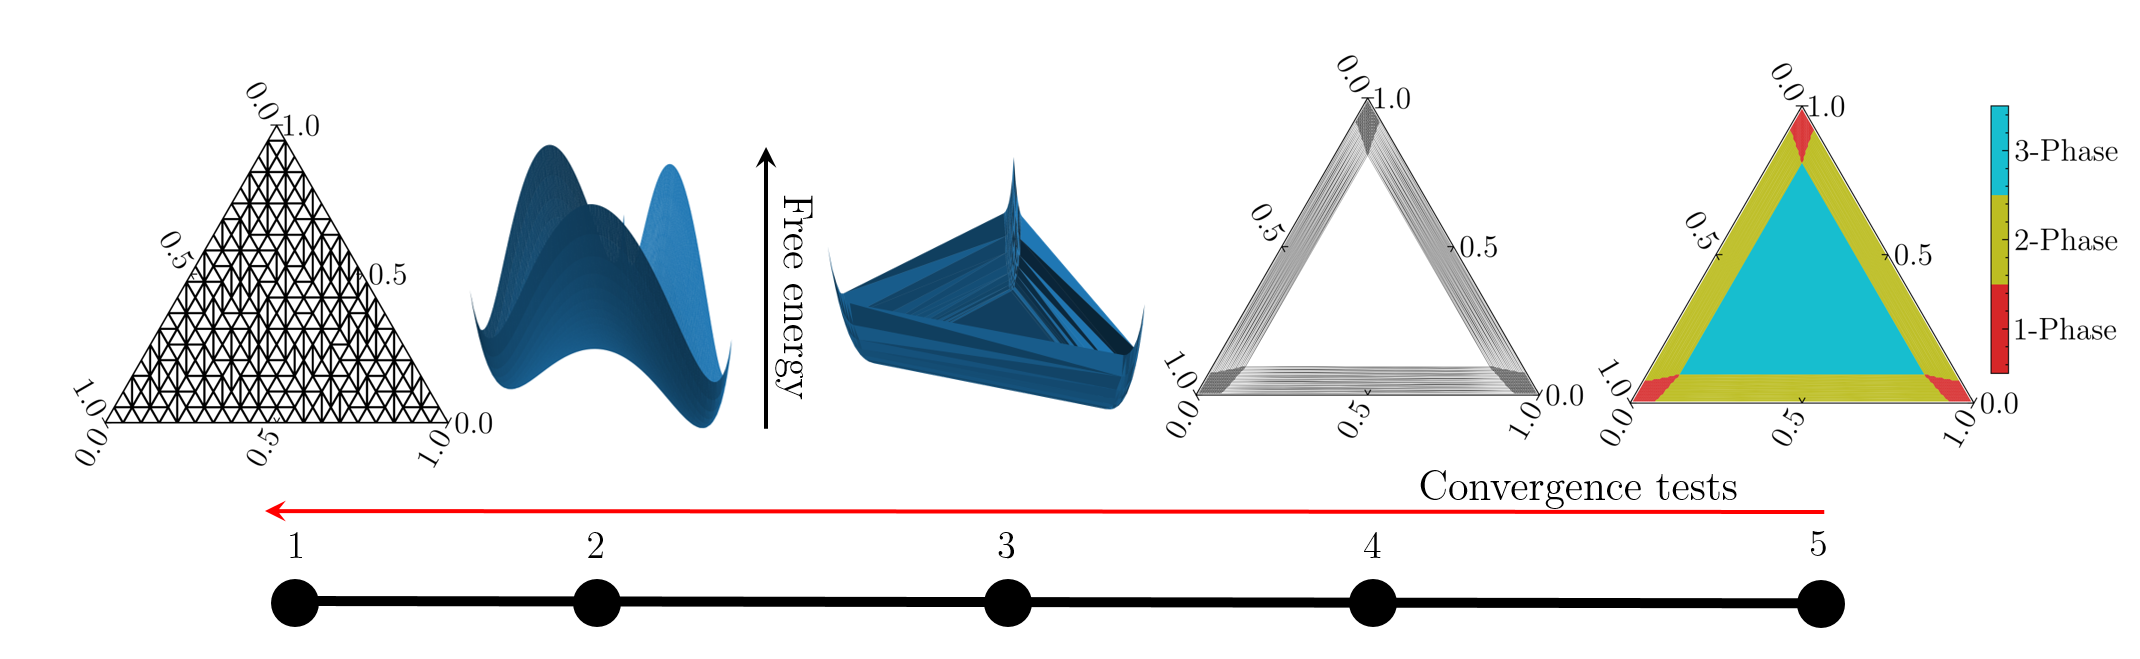
\includegraphics[width=\textwidth]{Chapter-4/figures/CEM_workflow.png}
    \caption{Convex envelope method visualized as a step-by-step process (1-5) with the series of tests performed. The red arrows depict where the tests can be performed and iterated until convergence, if required.}
    \label{fig:workflow}
\end{figure}

Two representations of phase diagrams are used:
The first representation corresponds to the output from~\Cref{algo:cem} and is referred as simplex-indexed set representation. 
The second representation is a a set indexed on the initial uniform grid $G$ (step 1 of~\Cref{algo:cem}), and is referred as a grid-indexed set representation.
The advantage of the second representation is the fixed size that ease the distance calculation. 
The grid-indexed representation is obtained from the simplex-indexed representation by assigning the phase label for each point in the grid by mapping it to the corresponding simplex in the convex envelope. 
The grid-indexed representation is used for the data analysis in~\Cref{sec:pipeline} and differentiate it from its simplex-indexed representation by a change of color-code while visualizing the phase diagram.

\section{Data generation}~\label{sec:htedata}
In ~\Cref{sec:pipeline}, a data-analysis pipeline is described to be applied on a relatively large sets of phase diagrams data described in~\Cref{sec:htedata}.
To derive the design rules we first perform dimensionality reduction followed by clustering. A overview of the dimensionality reduction and clustering methods can be found in~\ref{appendixB}.

The design space of variables are interaction parameter \(\chi\) values in~\Cref{eq:FH}.
The test case involves uniformly sampling the \(\chi\) values to be used in~\Cref{eq:FH} for a three component system. 
A uniform three-dimensional design space is defined via \(\chi_{12}\in[1.3,1.335,1.37,1.405,1.44]\) and 
\(\chi_{13}, \chi_{23}\in[0.3,0.6,1,1.5,2,2.5,3]\) a total of 245 phase diagrams are generated using the CEM method described in~\Cref{algo:cem}. 
The degree of polymerization for three materials are kept constant: $M_1=10$ for polymer, $M_2=10$ for small molecule, $M_3=1$ for solvent.
The goal using the model data set is to study the following question: \textit{given a densely sampled design space of phase diagram, can we automatically group various types of phase diagrams in the data set using clustering?}

\section{Data analysis pipeline}\label{sec:pipeline}
The data analysis pipeline as depicted in~\Cref{fig:mlpipeline} is as follows:~a) Generate a set of phase diagrams using the CEM in a high-throughput manner;~b) Compute pairwise similarities are and store in a matrix \(M\);~c) Apply clustering and dimensionality reduction to \(M\).
Spectral clustering method is used to obtain subgroups that are highly correlated within but not across using a Gaussian similarity of \(M\)~\cite{SpectralClustering}. 
A multi-dimensional scaling~(MDS)~\cite{ESL} of \(M\) is used to obtain a lower-dimensional representation using eigenvalues of \(M\) where each phase diagram can be represented using a point in a Cartesian coordinate system.
MDS and spectral clustering are performed using the \textit{scikit-learn}~\cite{sklearn} and other dependent python packages: scipy~\cite{scipy}, matplotlib~\cite{matplotlib} and mpltern~\cite{mpltern}.
Analyzing the lower dimensional representations and clustered subgroups together, allows users to decipher potential design rules that connect any two subgroups of phase diagrams. In \Cref{appendixB}, a detailed description of dimensionality reduction and clustering is provided with emphasis on geometrical interpretation of the methods used in this thesis.

The key element of the pipeline is the choice of the distance or similarity measure. The most commonly used distance is Euclidean norm, but other distances have been used~\cite{FiftySix}. 
In this work, we chose a \textit{Hamming} distance~(\Cref{eq:hamming}) between two grid-indexed representation of phase diagrams.

The point indexed phase diagram vectors are visualized by color-coding each point (instead of each simplex as before) in red (1-phase), green (2-phase) and blue (3-phase) as shown in (a) of~\Cref{fig:mlpipeline}.
The distance is then computed between a pair of phase label sets \(u,v\) indexed by composition using~\Cref{eq:hamming}.
\begin{equation}\label{eq:hamming}
    d(u,v) = \frac{1}{\ell}\sum_{i}\delta_{u[i],v[i]}
\end{equation}
where \(\delta_{ij}\) is the Kronecker-delta function and \(\ell\) is the cardinality of sets \(u,v\).
The Hamming distance is agnostic to the dimensionality of the grid \(G\), easy to compute thus making it a good choice for phase diagrams.  

\begin{figure}[h]
    \centering
    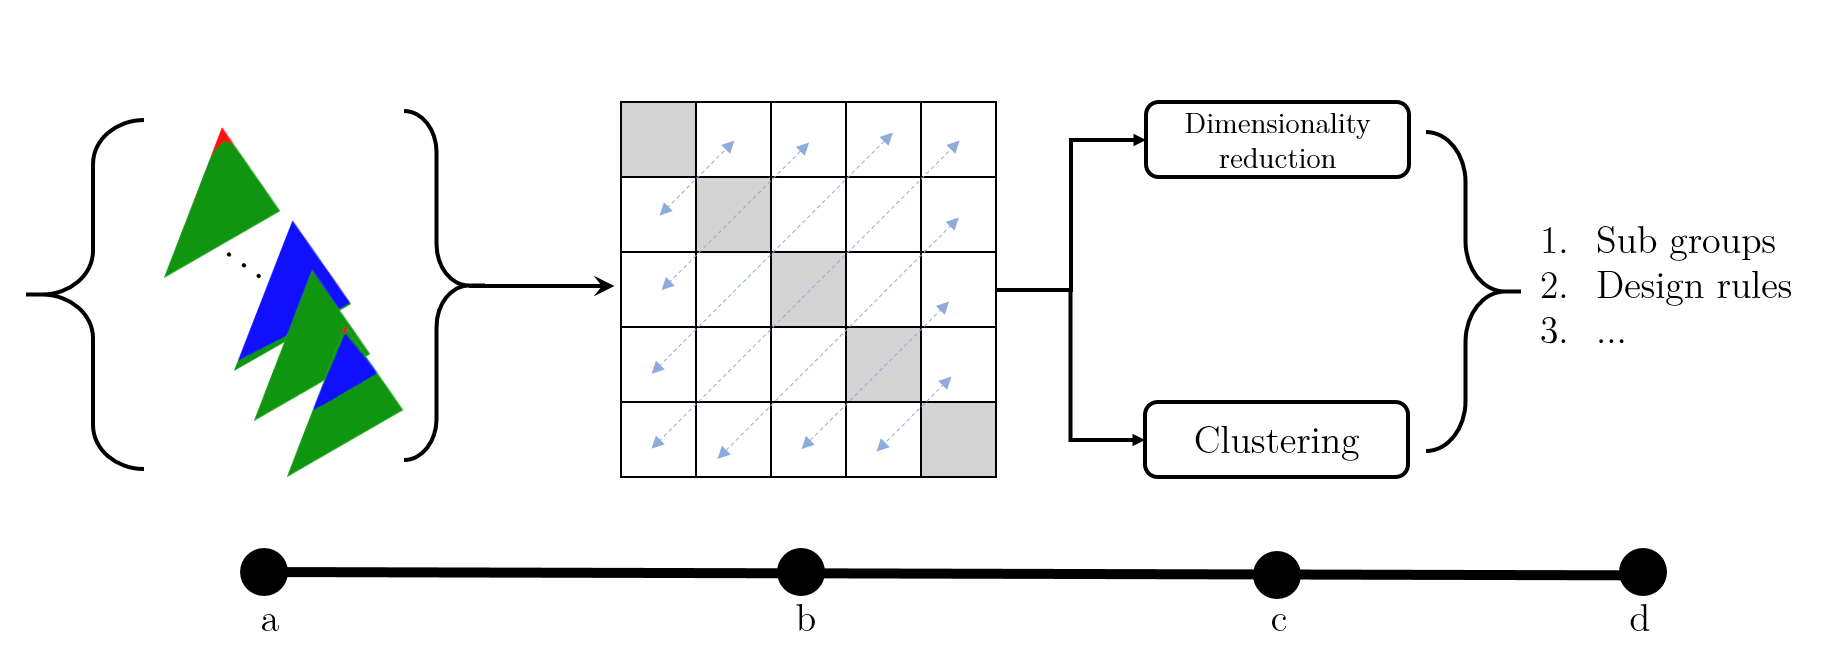
\includegraphics[width=\textwidth]{Chapter-4/figures/analysis_pipepline.png}
    \caption{Data analysis pipeline}
    \label{fig:mlpipeline}
\end{figure}


\section{Results and Discussions}\label{sec:results}
\subsection{Clustering phase diagrams}\label{sec:res:ct1}
\Cref{fig:result2_synthetic_mds} depicts a two-dimensional representation obtained using MDS with each point corresponding to a phase diagram in the model data set. 
The points are color-coded based on their spectral clustering labels (with a total of five clusters).
In \Cref{fig:result2_synthetic_clusters} we show the representative phase diagrams for each cluster. 
We observe that clusters in~\Cref{fig:synthdata} have distinct features: phase diagrams without any three phase regions (cluster 0); dominant in three phase region (cluster 1); all compositions belonging to three phase (cluster 2); mix of two and three phase regions (cluster 3,4) that differ in the direction of the phase boundary.
It is difficult to determine a way to obtain true clusters: We do more of a context-driven clustering where the hamming distance and number of clusters justify the true/real clusters (See section 5.3 in \cite{TrueClusters}).
In~\Cref{fig:synth_designspace}, we depict the \(\chi\) space sampling as points with \(\chi_{12},\chi_{13}, \chi_{23}\) as coordinate axes. 
The points are then colored based on the clustering label shown in \Cref{fig:result2_synthetic_mds}.
One can observe that the clusters show a radially evolving arrangement, which can be clearly seen in the two-dimensional projection of the design space shown in~\Cref{fig:synth_designspace_2D}.

\begin{figure}[h]\label{fig:synthdata}
    \centering
    \begin{subfigure}[b]{0.48\textwidth}
        \centering
        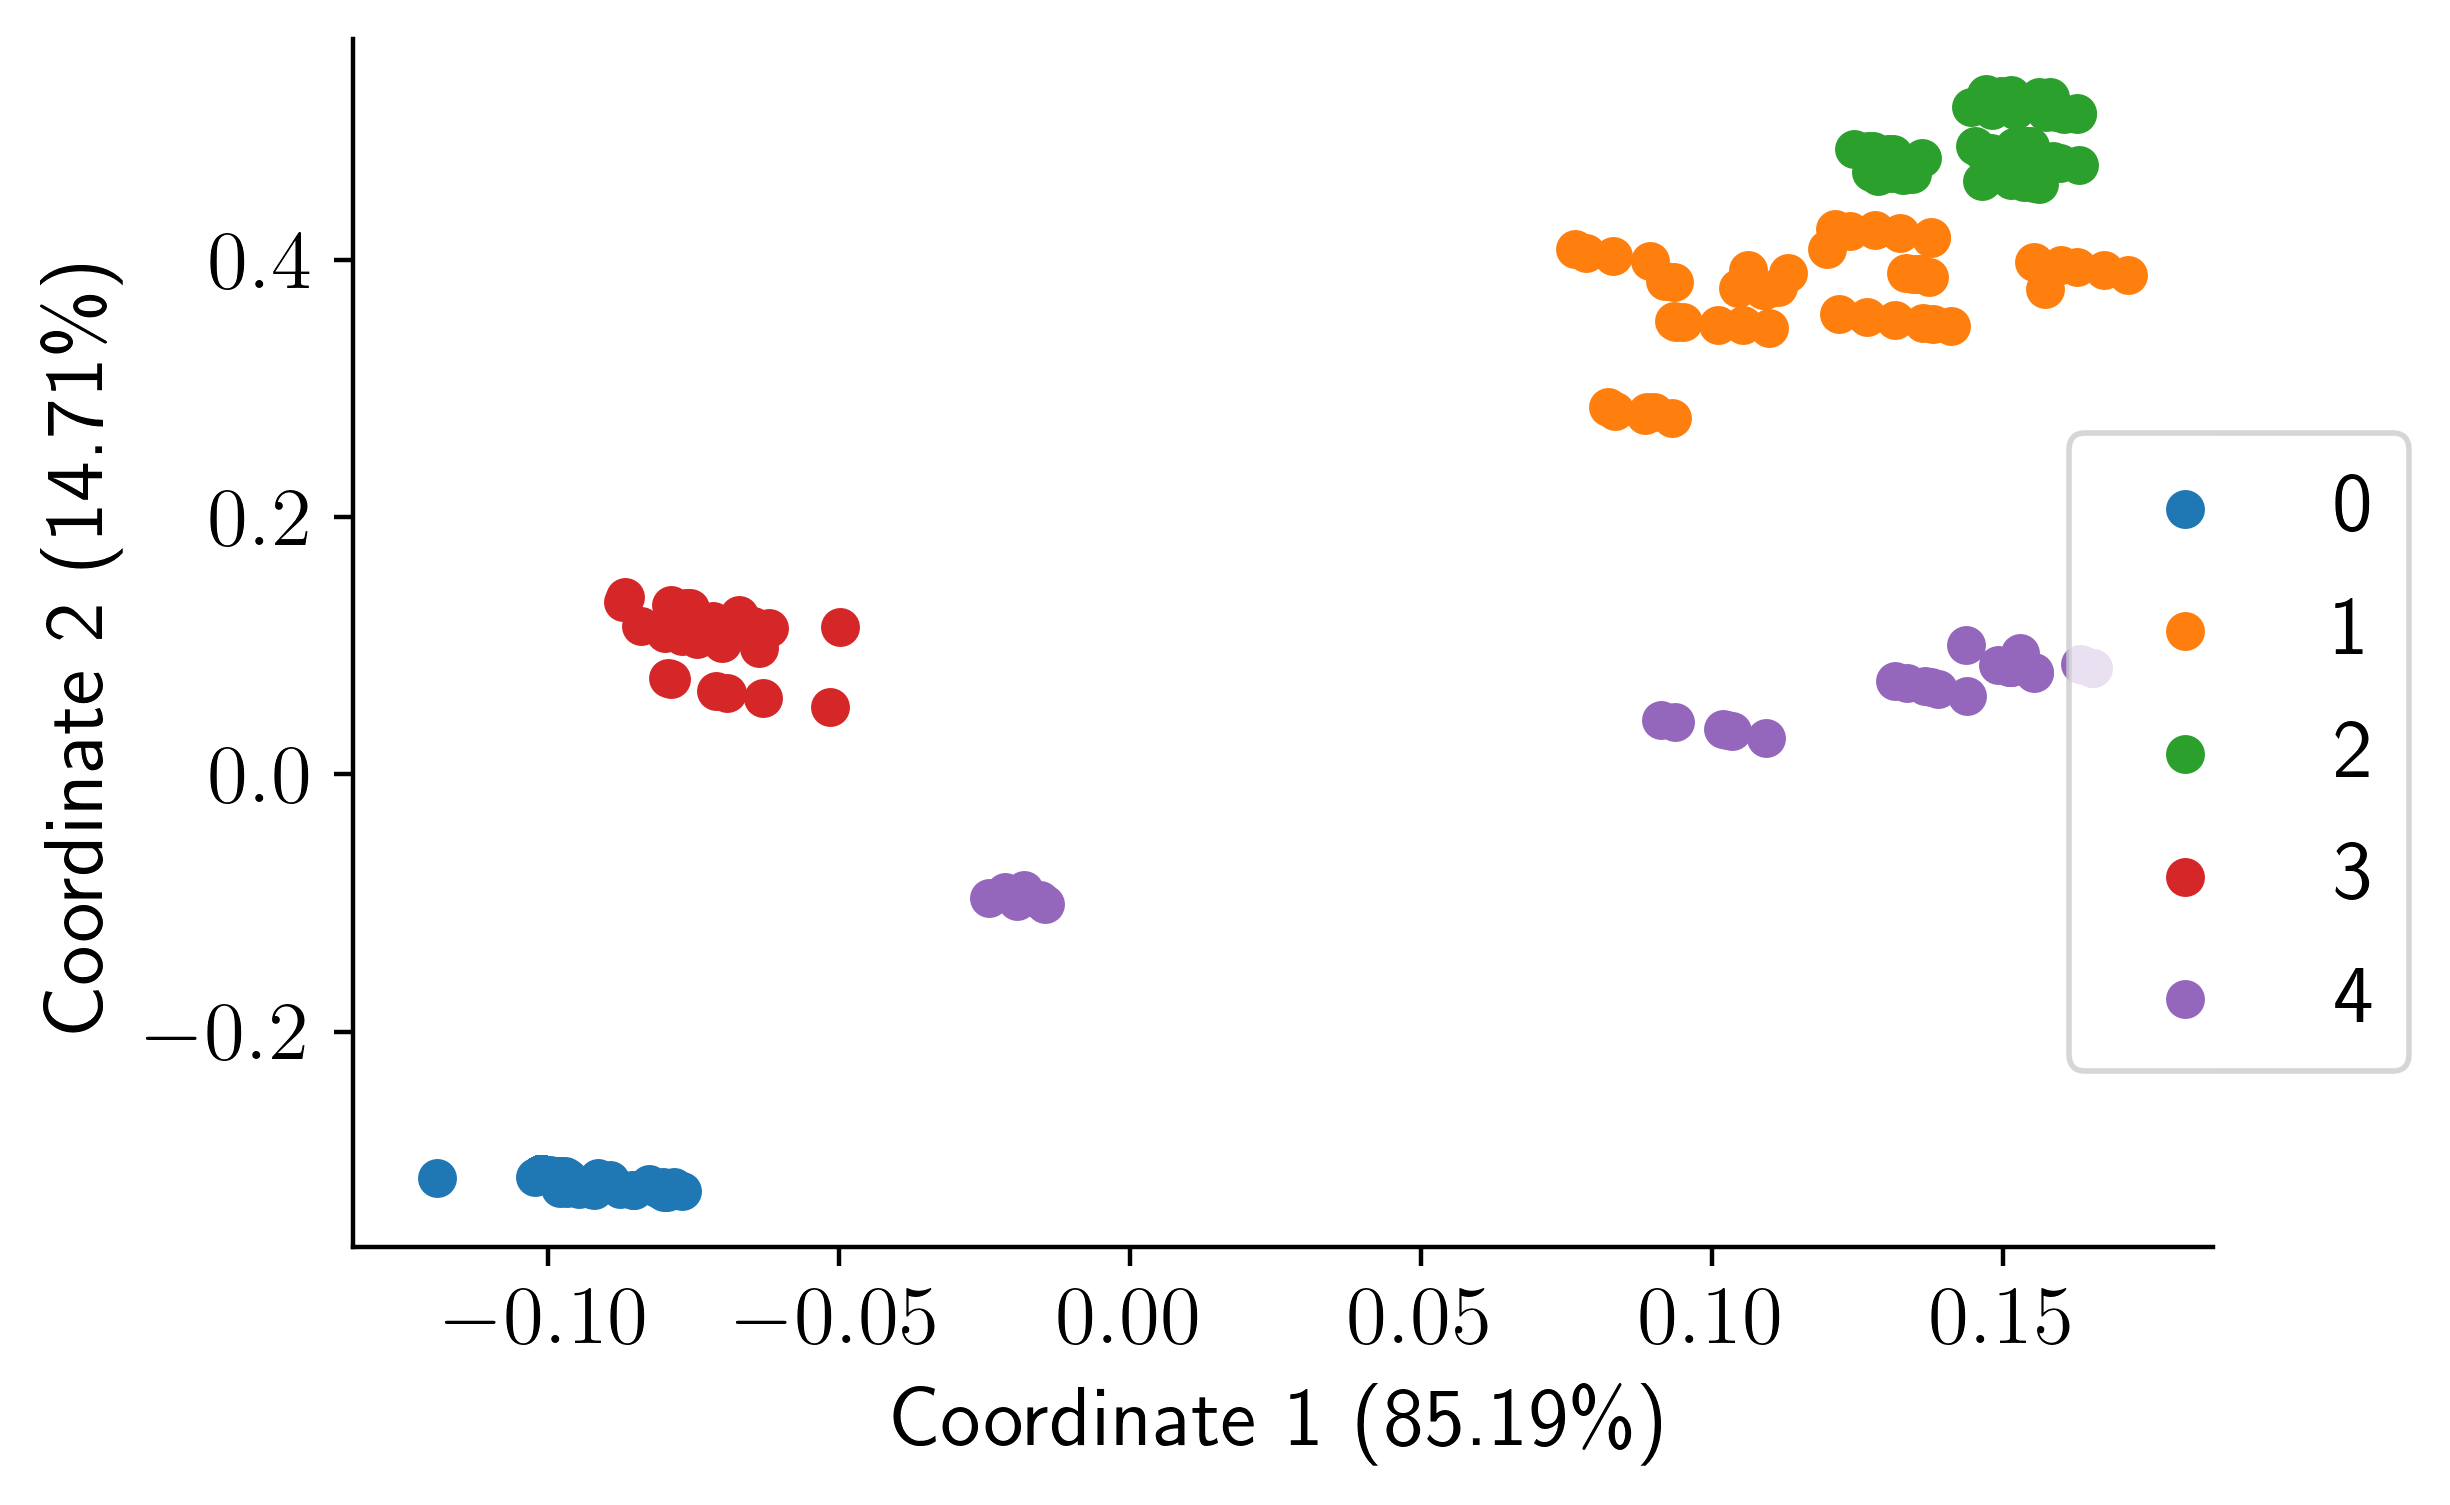
\includegraphics[width=\textwidth]{Chapter-4/figures/result2/result2_Synthetic_MDS.png}
        \label{fig:result2_synthetic_mds}
    \end{subfigure}
    \hfill
    \begin{subfigure}[b]{0.48\textwidth}
        \centering
        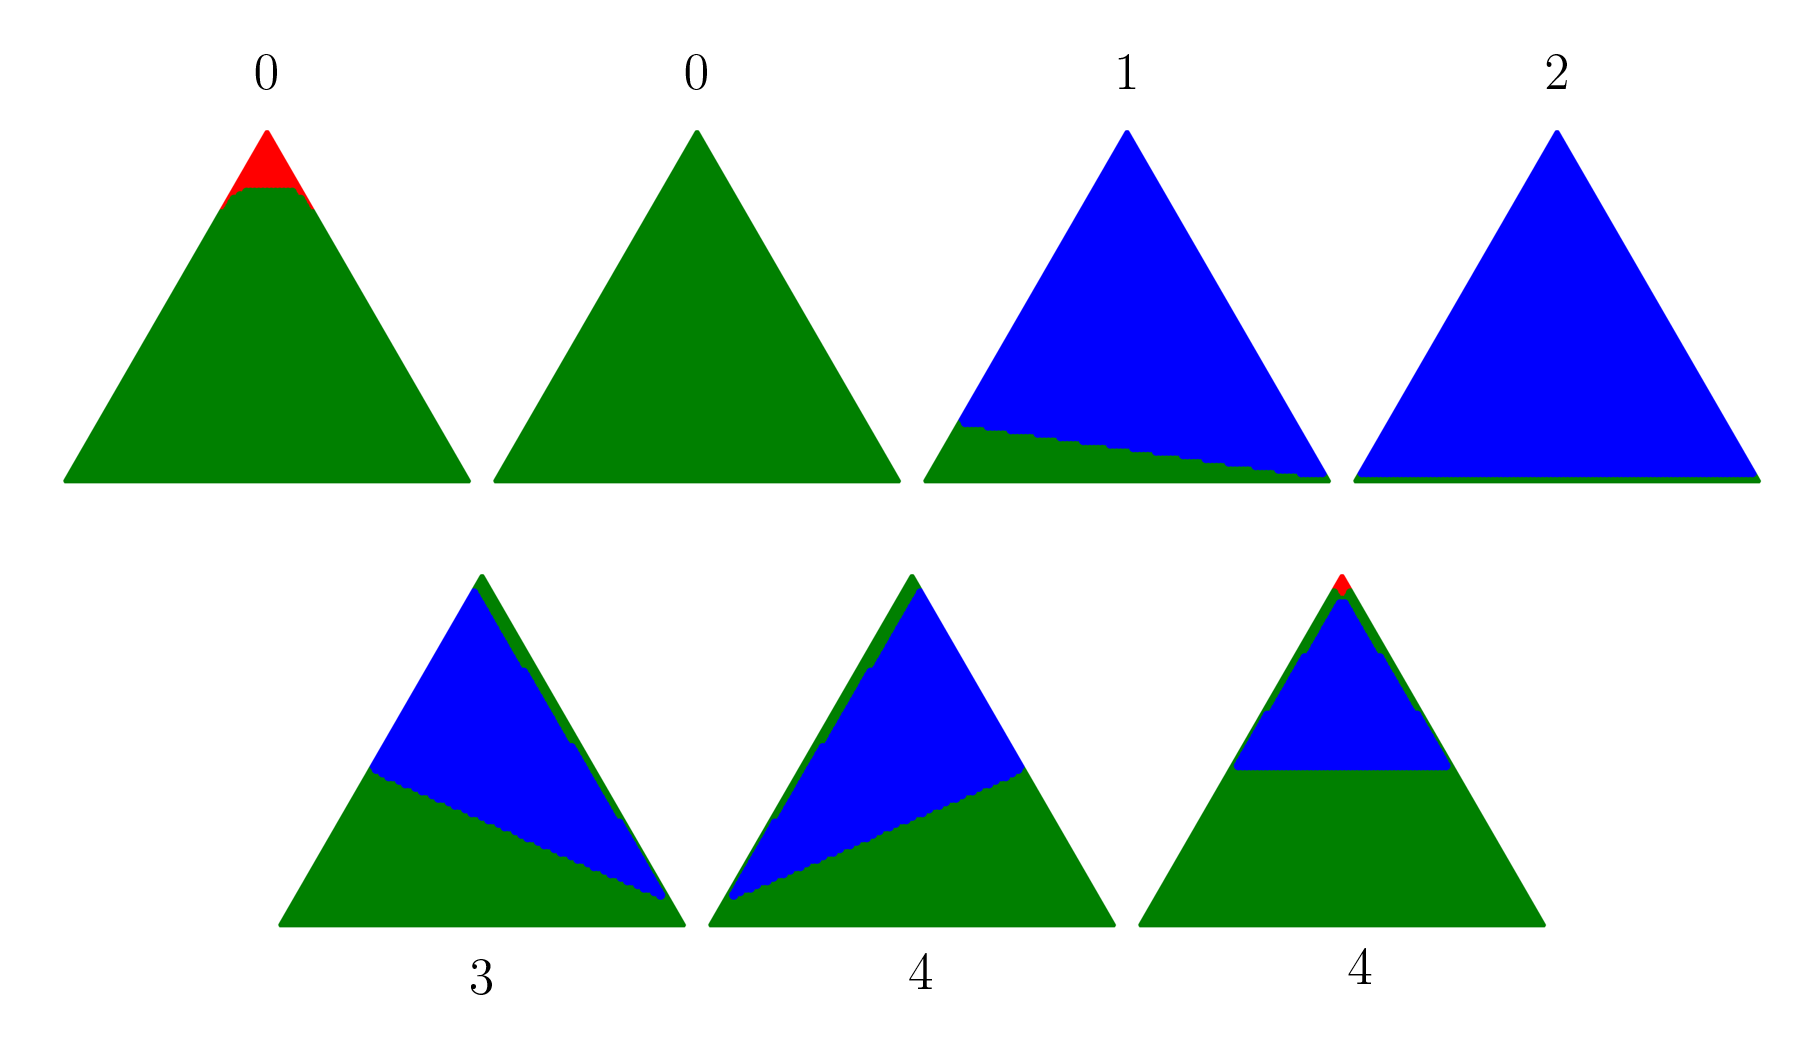
\includegraphics[width=\textwidth]{Chapter-4/figures/result2/result2_synthetic_clusters_manual.png}
        \caption{}
        \label{fig:result2_synthetic_clusters}
     \end{subfigure}
    \caption{Application of data analysis pipeline in \Cref{fig:mlpipeline} to mode data set in \Cref{sec:htedata}. (a) The lower dimensional Euclidean representation of the distance metric \(M\) for the space of 245 phase diagrams obtained for dataset presented in~\Cref{sec:htedata} using MDS. The color-code corresponds to the spectral clustering label. (b) Representative phase diagrams of clusters obtained from spectral clustering of metric \(M\). See text above for the discussion.}
\end{figure}

\begin{figure}[h]
    \centering  
    \begin{subfigure}[b]{0.4\textwidth}
        \centering
        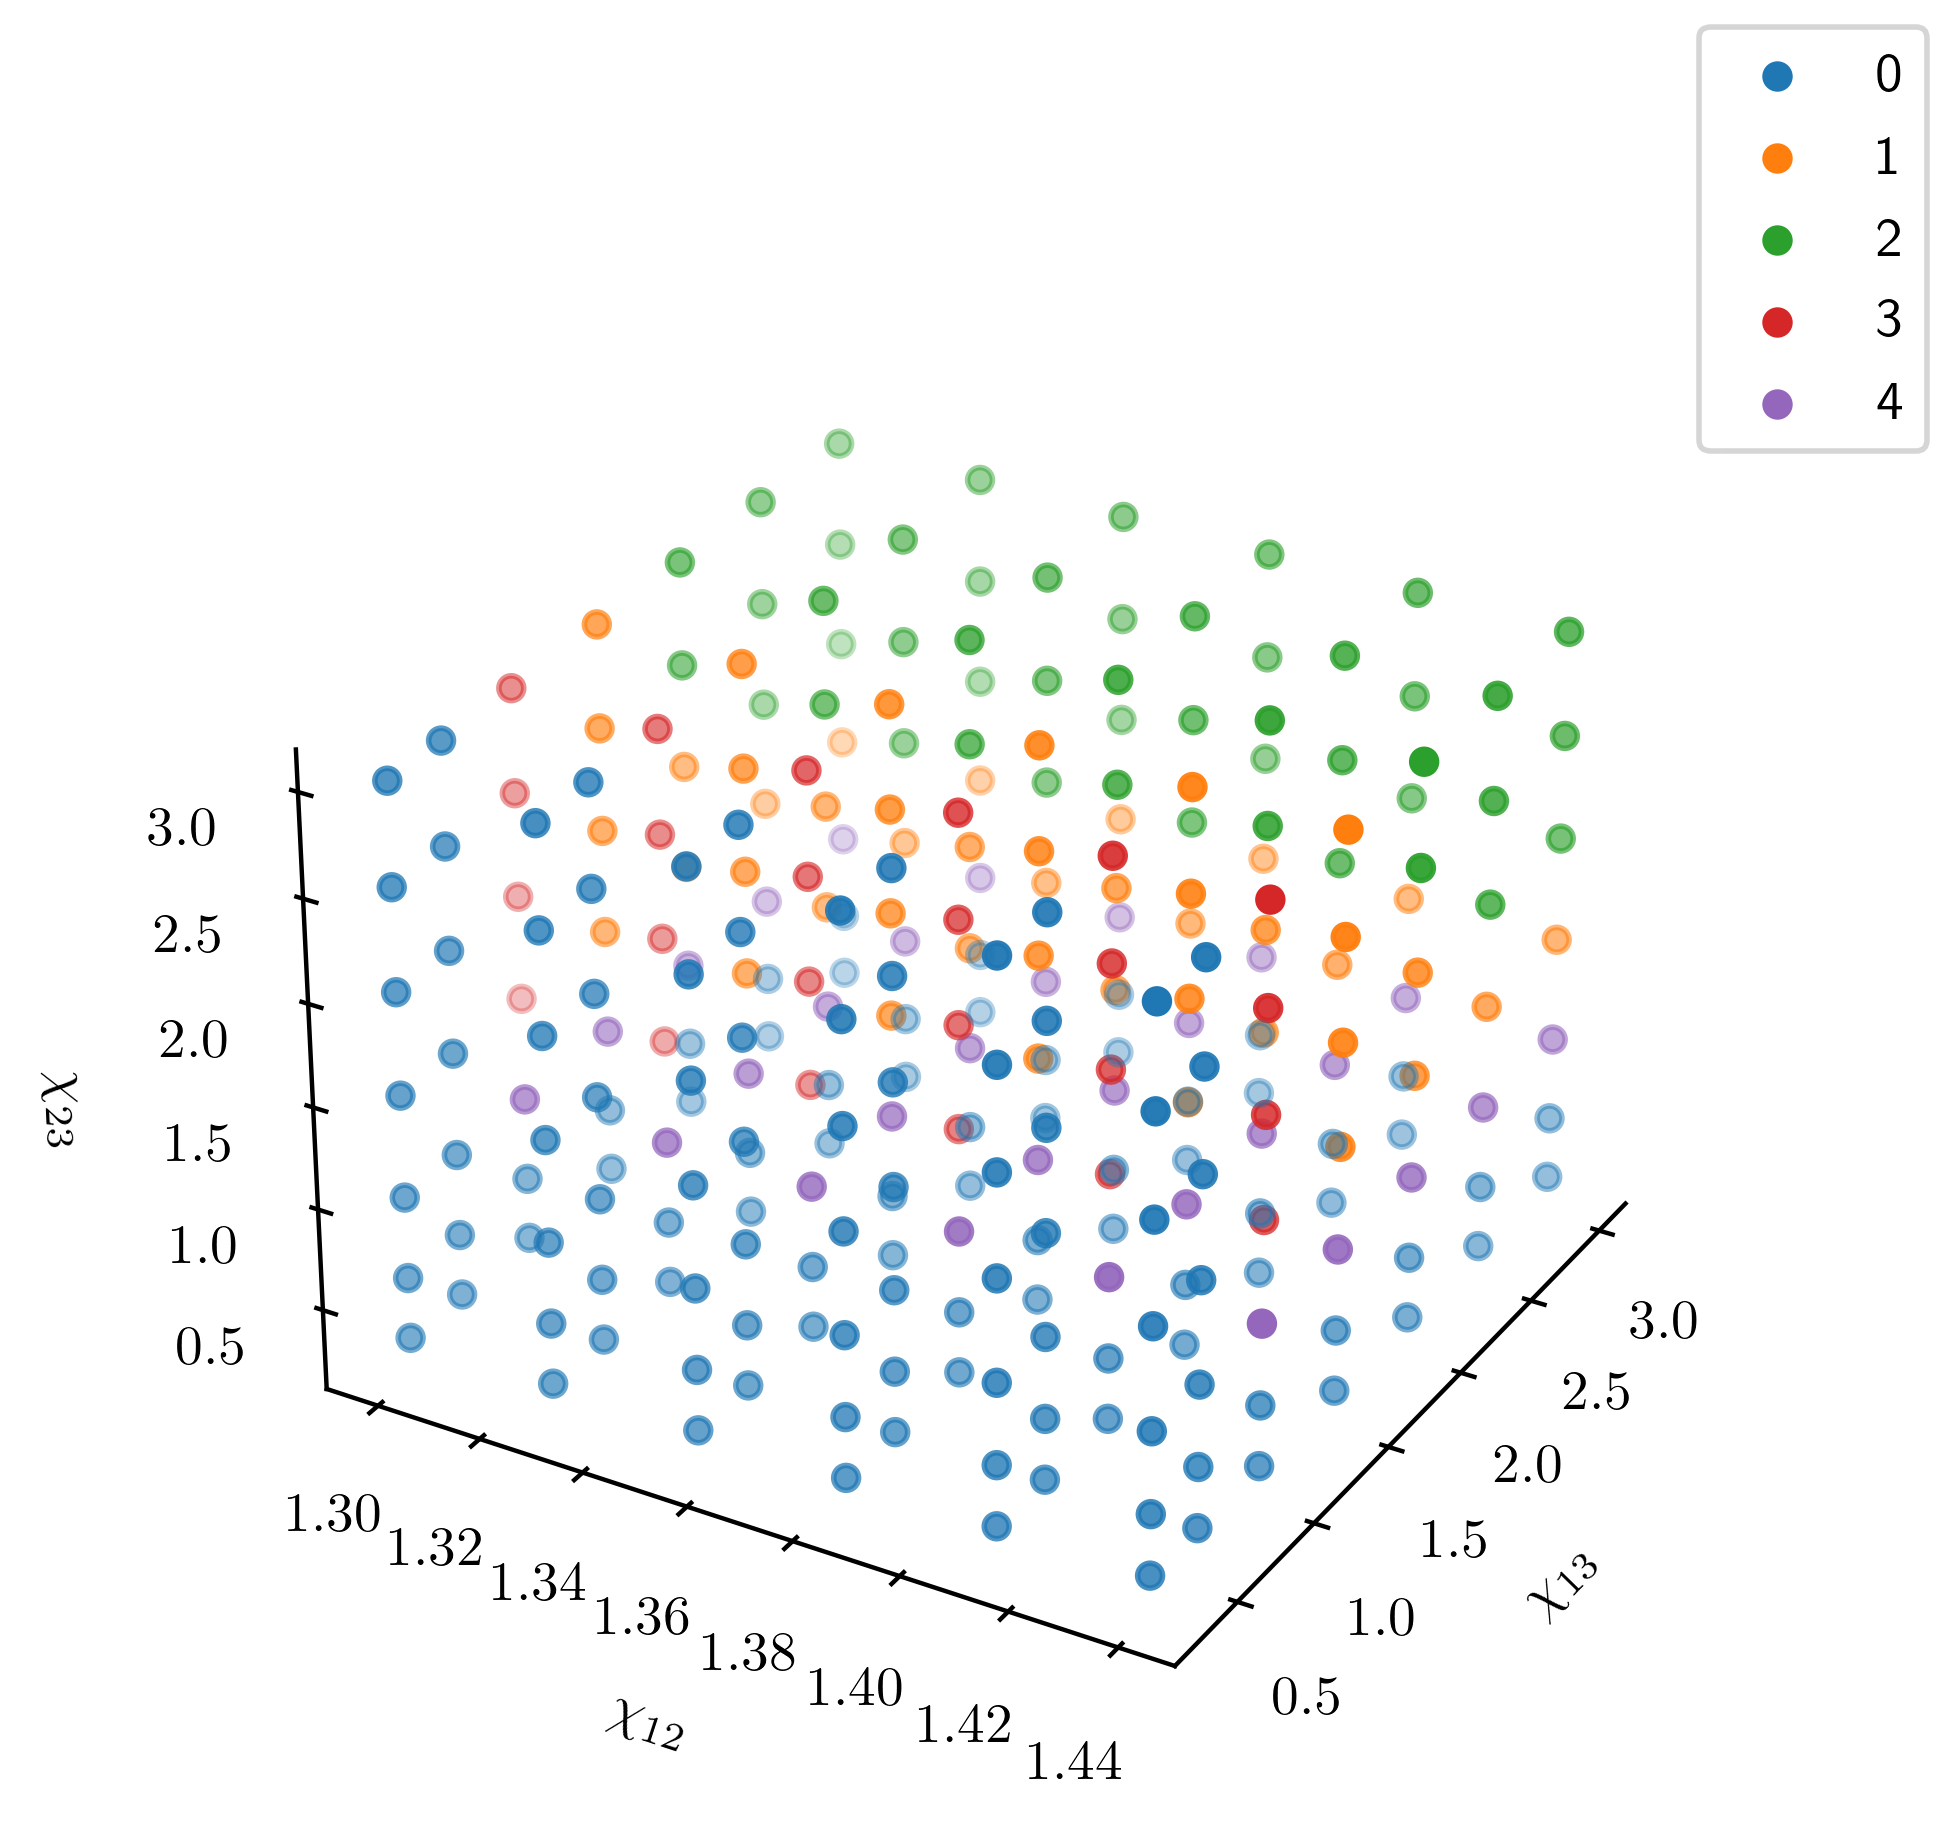
\includegraphics[width=\textwidth]{Chapter-4/figures/result2/result2_Synthetic_DesignSpace.png}
        \caption{}
        \label{fig:synth_designspace_3D}
    \end{subfigure}
    \hfill
    \begin{subfigure}[b]{0.4\textwidth}
        \centering
        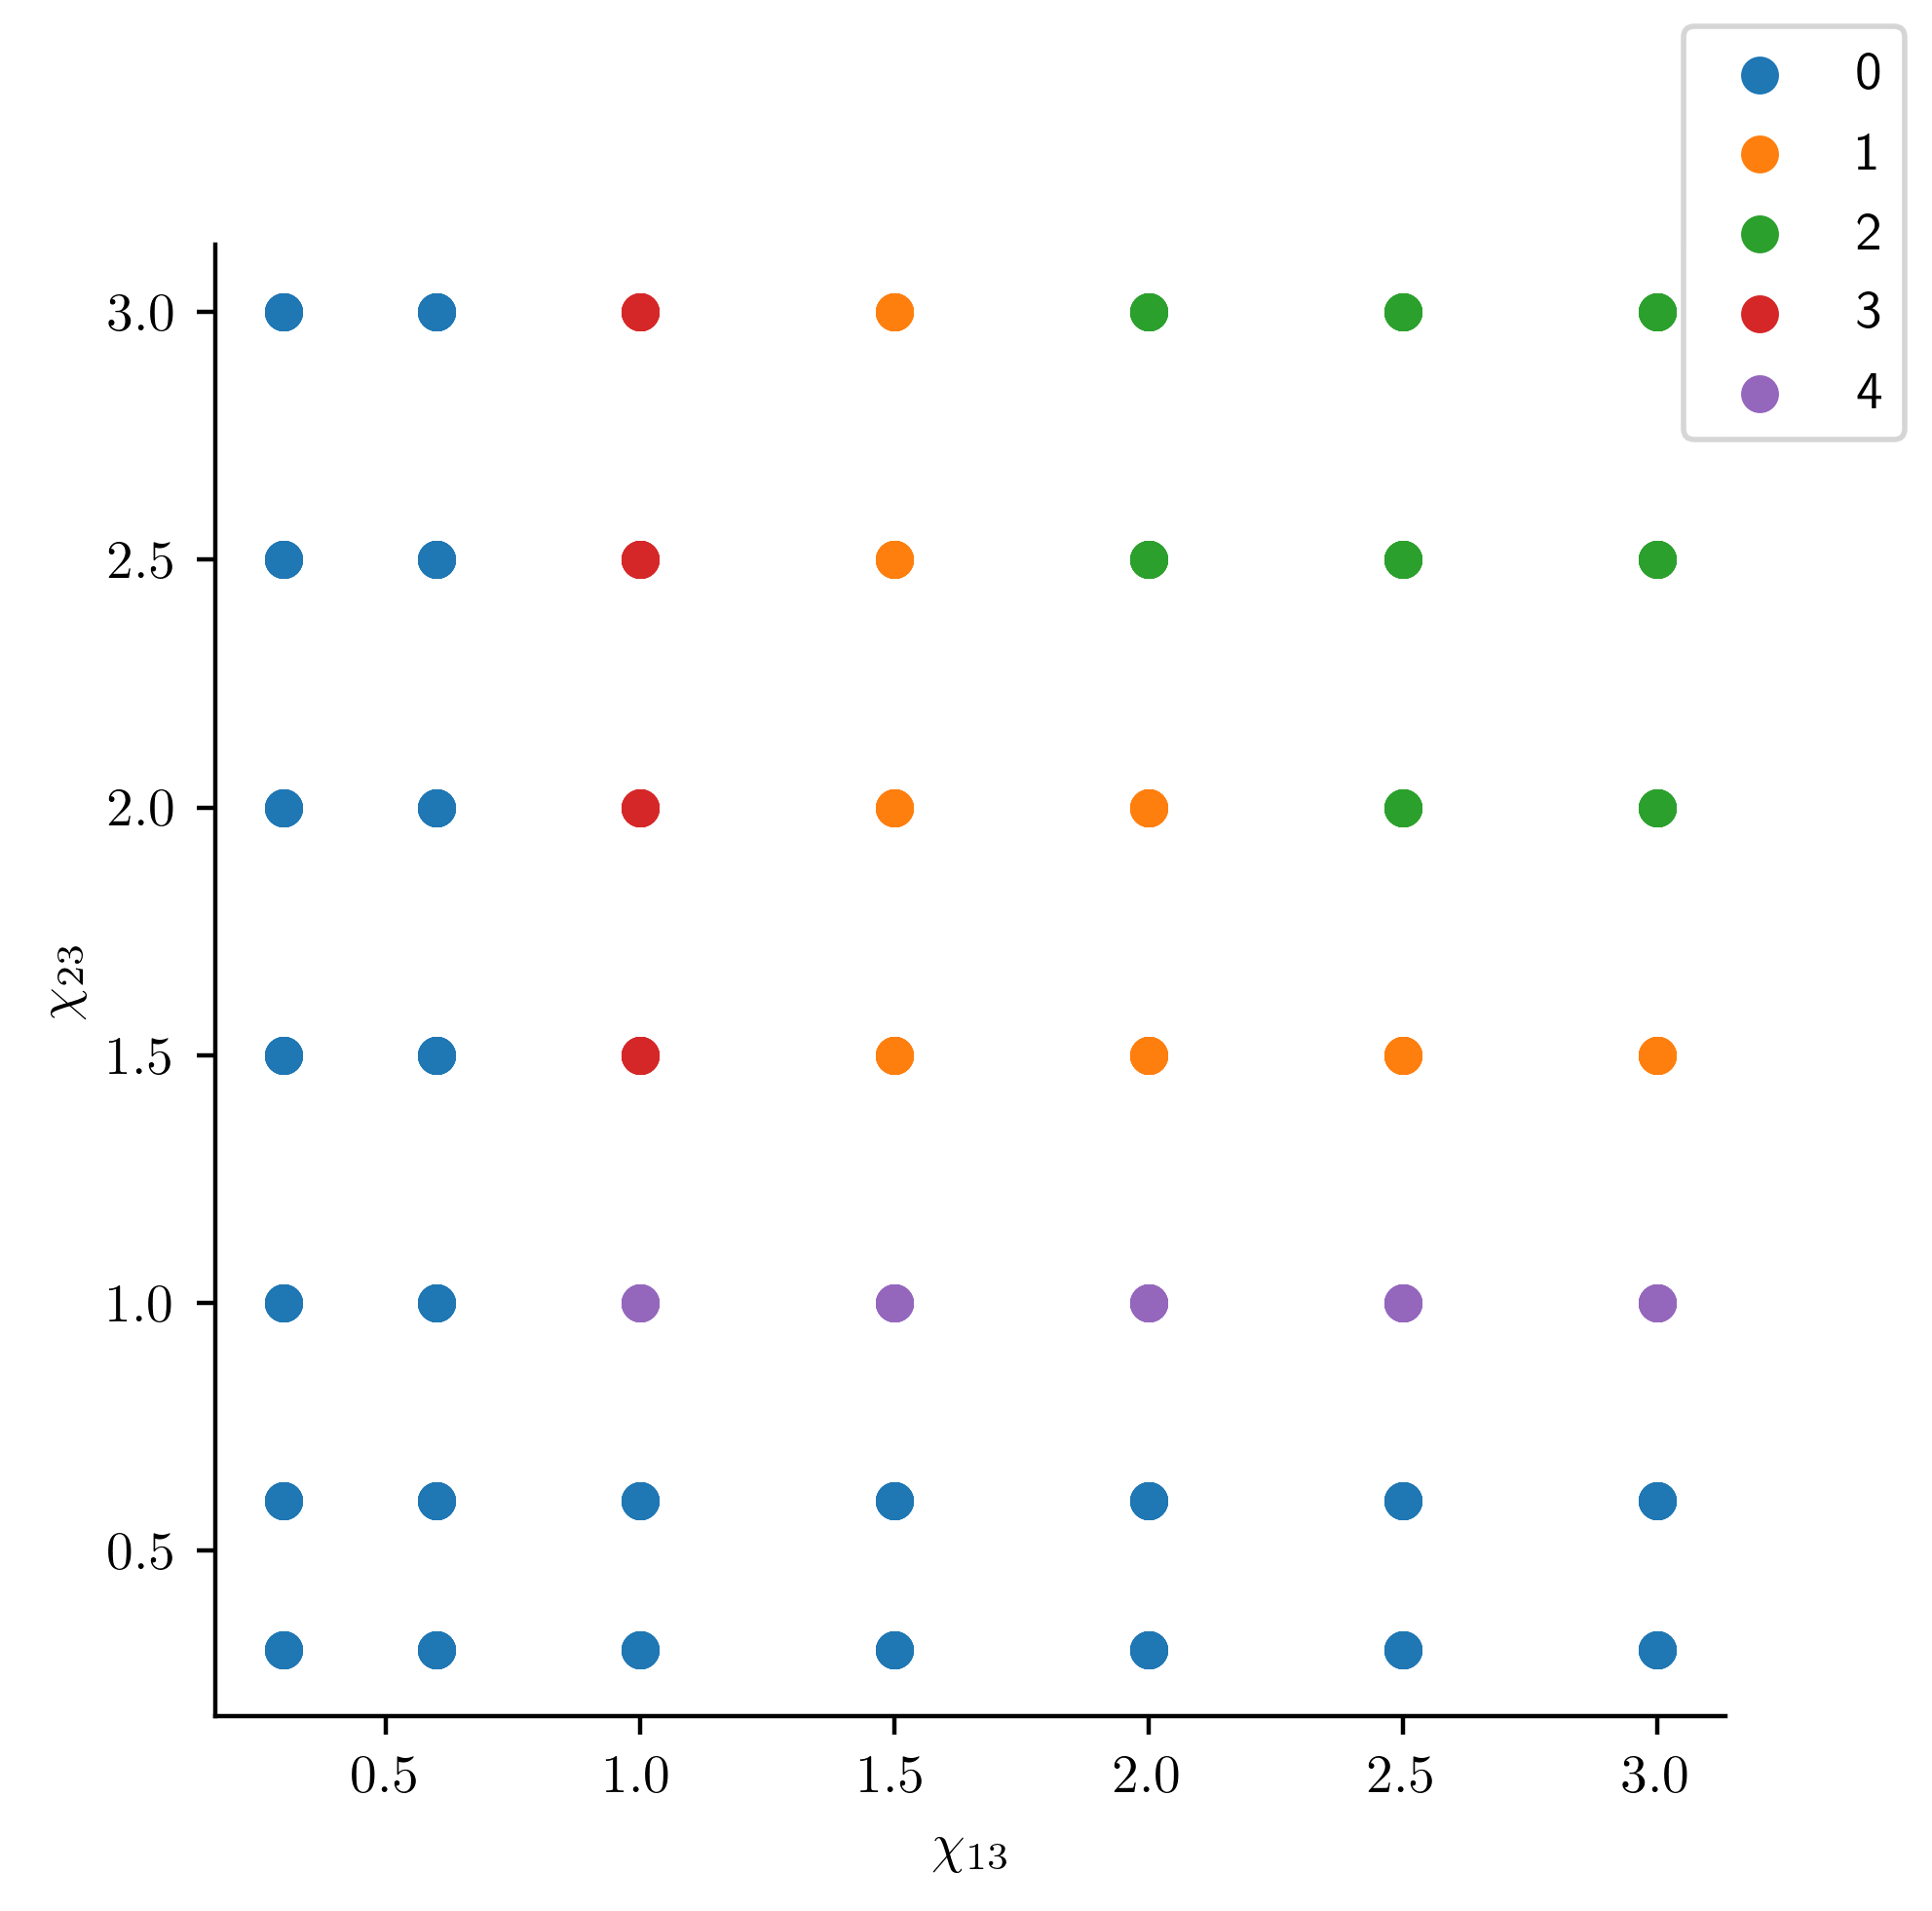
\includegraphics[width=\textwidth]{Chapter-4/figures/result2/result2_Synthetic_DesignSpace_2D.png}
        \caption{}
        \label{fig:synth_designspace_2D}
     \end{subfigure}
    \caption{Design space for model systems data set with points are color-coded with corresponding the cluster index of the phase diagram corresponds. (a) Input sampling space with \(\chi\) values as coordinates.Each point is colored based on their corresponding clustering label. (b) A radial trend in the clusters can be observed when visualizing the clusters on a two-dimensional projection of only \(\chi_{13}, \chi_{23}\).}
    \label{fig:synth_designspace}
\end{figure}

\section{Conclusions}
In this chapter, a high-throughput framework is introduced for phase diagram generation with the capabilities to evaluate for physical and computational accuracy. 
A data-analysis pipeline is used to perform initial screening of materials to identify subgroups there by decreasing the number of samples to be studied by an expert.
Applying the proposed methodology on two sets of material systems a framework is provided to derive potential design rules for solvent selection in OSC manufacturing.

